% Title: gl2ps_renderer figure
% Creator: GL2PS 1.4.2, (C) 1999-2020 C. Geuzaine
% For: Octave
% CreationDate: Thu Aug  8 09:06:37 2024
\setlength{\unitlength}{1pt}
\begin{picture}(0,0)
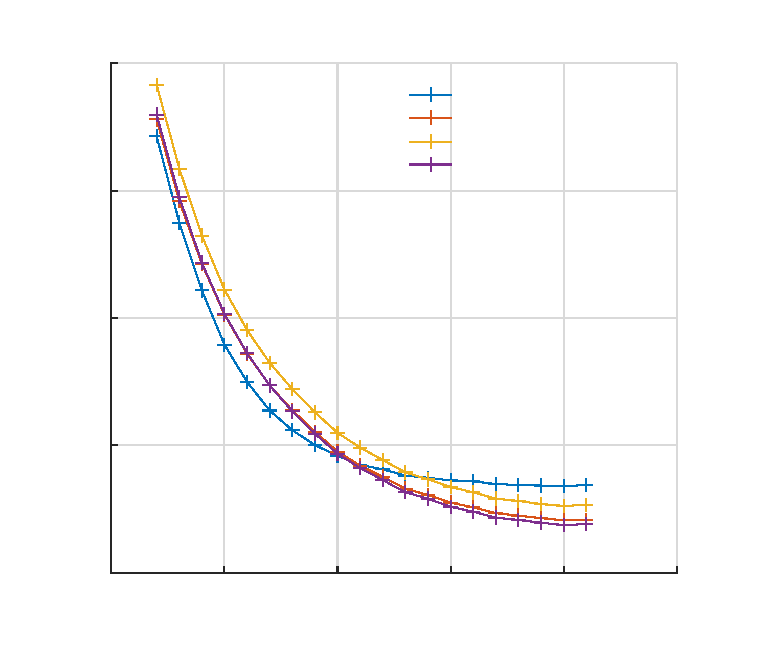
\includegraphics[scale=1]{loss_EqNo_models-inc}
\end{picture}%
\begin{picture}(350,300)(0,0)
\fontsize{7}{0}\selectfont\put(45.5,27.54){\makebox(0,0)[t]{\textcolor[rgb]{0.15,0.15,0.15}{{-5}}}}
\fontsize{7}{0}\selectfont\put(99.75,27.54){\makebox(0,0)[t]{\textcolor[rgb]{0.15,0.15,0.15}{{0}}}}
\fontsize{7}{0}\selectfont\put(154,27.54){\makebox(0,0)[t]{\textcolor[rgb]{0.15,0.15,0.15}{{5}}}}
\fontsize{7}{0}\selectfont\put(208.25,27.54){\makebox(0,0)[t]{\textcolor[rgb]{0.15,0.15,0.15}{{10}}}}
\fontsize{7}{0}\selectfont\put(262.5,27.54){\makebox(0,0)[t]{\textcolor[rgb]{0.15,0.15,0.15}{{15}}}}
\fontsize{7}{0}\selectfont\put(316.75,27.54){\makebox(0,0)[t]{\textcolor[rgb]{0.15,0.15,0.15}{{20}}}}
\fontsize{7}{0}\selectfont\put(41.8491,33){\makebox(0,0)[r]{\textcolor[rgb]{0.15,0.15,0.15}{{0.05}}}}
\fontsize{7}{0}\selectfont\put(41.8491,94.125){\makebox(0,0)[r]{\textcolor[rgb]{0.15,0.15,0.15}{{0.1}}}}
\fontsize{7}{0}\selectfont\put(41.8491,155.25){\makebox(0,0)[r]{\textcolor[rgb]{0.15,0.15,0.15}{{0.15}}}}
\fontsize{7}{0}\selectfont\put(41.8491,216.375){\makebox(0,0)[r]{\textcolor[rgb]{0.15,0.15,0.15}{{0.2}}}}
\fontsize{7}{0}\selectfont\put(41.8491,277.5){\makebox(0,0)[r]{\textcolor[rgb]{0.15,0.15,0.15}{{0.25}}}}
\fontsize{8}{0}\selectfont\put(181.125,15.54){\makebox(0,0)[t]{\textcolor[rgb]{0.15,0.15,0.15}{{Eq/No (dB)}}}}
\fontsize{8}{0}\selectfont\put(22.8491,155.25){\rotatebox{90}{\makebox(0,0)[b]{\textcolor[rgb]{0.15,0.15,0.15}{{loss}}}}}
\fontsize{6}{0}\selectfont\put(212.755,262.443){\makebox(0,0)[l]{\textcolor[rgb]{0,0,0}{{m5 1D}}}}
\fontsize{6}{0}\selectfont\put(212.755,251.382){\makebox(0,0)[l]{\textcolor[rgb]{0,0,0}{{m17 check7 2D PAPR opt}}}}
\fontsize{6}{0}\selectfont\put(212.755,239.884){\makebox(0,0)[l]{\textcolor[rgb]{0,0,0}{{m19 m17 + aux data 1}}}}
\fontsize{6}{0}\selectfont\put(212.755,228.885){\makebox(0,0)[l]{\textcolor[rgb]{0,0,0}{{m19 check3 m17 + aux data 2}}}}
\end{picture}
